\section{Структуры данных и путешествия во времени} \noteauthoress{Татьяна Белова}

Оригинальная статья: \cite{demaine2007retroactive}.

В этом разделе нам будут интересны структуры данных, позволяющие осуществлять эти самые "путешествия во времени".
Определить это понятие можно по-разному, мы разберем два варианта: персистентность и ретрактивность.

\subsection{Персистентность} \label{sec:persist}

Мы будем рассматривать структуры данных в модели pointer machine.
Структура данных рассматривается как некоторое множество узлов, в каждом узле хранится $\mathcal{O}(1)$ полей, в поле может быть записано число или указатель на другой узел, смотреть Рисунок~\ref{fig:TanyaPM}.
Иногда вводят дополнительное константное ограничение на входящую степень узла, то есть, для каждого узла, количество указателей, указывающих на него, должно быть не больше какой-то константы.

\begin{figure}[h] \centering
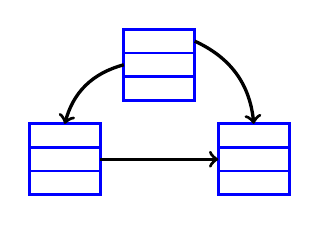
\begin{tikzpicture}[scale = 0.3]

\draw[blue, thick] (0,0) rectangle (3,1);
\draw[blue, thick] (0,0) rectangle (3,2);
\draw[blue, very thick] (0,0) rectangle (3,3);

\draw[blue, thick] (8,0) rectangle (11,1);
\draw[blue, thick] (8,0) rectangle (11,2);
\draw[blue, very thick] (8,0) rectangle (11,3);

\draw[blue, thick] (4,4) rectangle (7,5);
\draw[blue, thick] (4,4) rectangle (7,6);
\draw[blue, very thick] (4,4) rectangle (7,7);

\draw[very thick, ->] (4, 5.5) [bend right] to (1.5,3);
\draw[very thick, ->] (7, 6.5) [bend left] to (9.5, 3);
\draw[very thick, ->] (3, 1.5) to (8, 1.5);
\end{tikzpicture}
	\caption{Pointer machine}
	\label{fig:TanyaPM}
\end{figure}

\vspace{10pt}
Операции, которые поддерживает структура: 

\begin{itemize}

\item $x = $ new node --- создать новый узел
\item $x = y.$field --- взять значение поля
\item $x = y + z$ --- объединить два узла
\item destroy($x$) --- удалить узел, если на него нет указателя

\end{itemize}

Персистентность бывает разных видов:

\begin{enumerate}

\item {\bf Частичная персистентность}

\begin{itemize}

\item изменяем только последнюю версию
\item спрашиваем о любых версиях

\end{itemize}

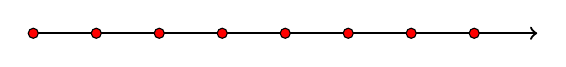
\begin{tikzpicture}[scale = 0.8]

\draw[thick, ->] (0,0) -- (8,0);


\foreach \x in {0, ..., 7}{
  \filldraw[fill=red] (\x, 0) circle (0.08);    
}

\end{tikzpicture}
\vspace{10pt}

{\it Известные результаты.} Если у структуры данных константная входящая степень для всех узлов, то можно сделать ее частично персистентной с константным мультипликативным overhead-ом.

\cite{driscoll1986making} сделали алгоритм с амортизированным $\mathcal{O}(1)$ overhead-ом.

\cite{brodal1996partially} сделали алгоритм с $\mathcal{O}(1)$ overhead-ом в худшем случае.

\item \label{item:fullPers} {\bf Полная персистентность}: частичная + можем изменять прошлое.

Каждый раз, когда мы изменяем прошлое, мы создаем новую версию структуры. Получается дерево версий, смотреть Рисунок~\ref{fig:TanyaTree}.

\begin{figure}[h] \centering
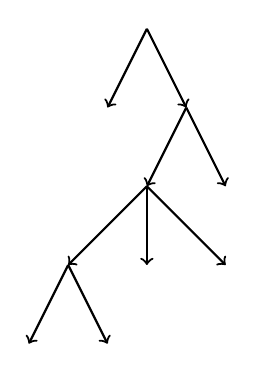
\begin{tikzpicture}[scale = 0.5]

\draw[thick, ->] (4,9) -- (3,7);
\draw[thick, ->] (4,9) -- (5,7);
\draw[thick, ->] (5,7) -- (6,5);
\draw[thick, ->] (5,7) -- (4,5);
\draw[thick, ->] (4,5) -- (6,3);
\draw[thick, ->] (4,5) -- (4,3);
\draw[thick, ->] (4,5) -- (2,3);
\draw[thick, ->] (2,3) -- (1,1);
\draw[thick, ->] (2,3) -- (3,1);

\end{tikzpicture}
	\caption{Полная персистентность}
	\label{fig:TanyaTree}
\end{figure}

{\it Известные результаты.} Если у структуры данных константная входящая степень для всех узлов, то ее можно наделить полной персистентностью также с константным мультипликативным overhead-ом. Правда в случае полной персистентности такого overhead-а умеют добиваться только амортизированно (\cite{driscoll1986making}), и можно ли добиться его в худшем случае --- открытый вопрос.  

\item {\bf Конфлюентная персистентность}: полная + можем комбинировать версии.

В этом случае, помимо обычных изменений структуры, можно также сливать две версии в одну. 
Получается ацикличный граф версий, смотреть Рисунок~\ref{fig:TanyaAcyc}.

\begin{figure}[h] \centering
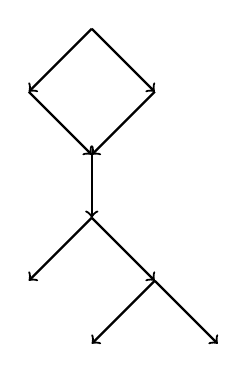
\begin{tikzpicture}[scale = 0.8]

\draw[thick, ->] (0,10) -- (-1,9);
\draw[thick, ->] (0,10) -- (1,9);
\draw[thick, ->] (-1,9) -- (0,8);
\draw[thick, ->] (1,9) -- (0,8);
\draw[thick, ->] (0,8) -- (0,7);
\draw[thick, ->] (0,7) -- (-1,6);
\draw[thick, ->] (0,7) -- (1,6);
\draw[thick, ->] (1,6) -- (0,5);
\draw[thick, ->] (1,6) -- (2,5);

\end{tikzpicture}
	\caption{Конфлюентная персистентность}
	\label{fig:TanyaAcyc}
\end{figure}


{\it Известные результаты.} С конфлюентной персистентностью все сложнее, \cite{fiat2003making} умеют с overhead-ом $\log(\#upd) + \max\limits_v e(v)$, 
где $\#upd$ -- это количество всех сделанных к этому моменту изменений, $v$ -- вершина в графе версий, а $e(v) = 1 + log\#$(путей из корня в $v$).

Открытый вопрос: можно ли сделать overhead $\mathcal{O}(\log n)$?
При этом $\mathcal{O}(\log n)$ умеют получать для частного случая задачи, когда мы хотим сливать только версии, в которых нет общих полей (\cite{collette2012confluent}).

\item {\bf Функциональная персистентность}: комбинированная + нельзя модифицировать узлы

{\it Известные результаты.} В общем виде задачу решать не умеют.
Умеют только для частных случаев. Например, Balanced BST и Link-cut-tree умеют делать функционально персистентными с overhead-ом $\mathcal{O}(\log n)$ (\cite{demaine2008confluently}).

\end{enumerate}

\subsection*{Приложения частичной персистентности}

{\bf Задача Point location}

Дан плоский граф $G$ с ребрами-отрезками.
Запросы: по данной точке определить, в какой грани она находится.
Можно сделать предобработку. 

%\vspace{10pt}
%\begin{tikzpicture}[scale = 0.5]

%\draw[thick] (3,4) -- (9,2);
%\draw[thick] (3,4) -- (5,7);
%\draw[thick] (3,4) -- (2,9);
%\draw[thick] (2,9) -- (4,13);
%\draw[thick] (2,9) -- (5,7);
%\draw[thick] (5,7) -- (7,7);
%\draw[thick] (4,13) -- (12,13);
%\draw[thick] (4,13) -- (8,11);
%\draw[thick] (7,7) -- (8,11);
%\draw[thick] (7,7) -- (11,5);
%\draw[thick] (8,11) -- (12,13);
%\draw[thick] (9,2) -- (11,5);
%\draw[thick] (11,5) -- (12,13);

%\draw [fill] (6,10) circle [radius=0.1];
%\node (q) at (6.5,10) {$q$};

%\end{tikzpicture}

{\bf Решение с помощью частичной персистентности.}

Отсортируем вершины графа по координате $x$. 
Будем в этом порядке добавлять вершины и поддерживать множество ребер, которые пересекают вертикальную полоску от этой вершины до следующей.
Ребра будем хранить в каком-нибудь BST.
Таким образом, у нас появилось $n$ версий этого BST, по версии для каждой точки, смотреть Рисунок~\ref{fig:TanyaBST}.

\begin{figure}[h] \centering
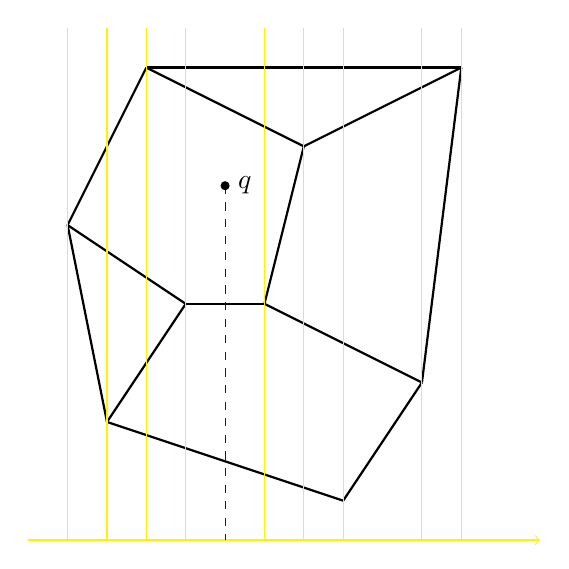
\begin{tikzpicture}[scale = 0.5]

\draw[thick] (3,4) -- (9,2);
\draw[thick] (3,4) -- (5,7);
\draw[thick] (3,4) -- (2,9);
\draw[thick] (2,9) -- (4,13);
\draw[thick] (2,9) -- (5,7);
\draw[thick] (5,7) -- (7,7);
\draw[thick] (4,13) -- (12,13);
\draw[thick] (4,13) -- (8,11);
\draw[thick] (7,7) -- (8,11);
\draw[thick] (7,7) -- (11,5);
\draw[thick] (8,11) -- (12,13);
\draw[thick] (9,2) -- (11,5);
\draw[thick] (11,5) -- (12,13);

\foreach \x in {2,3,4,5,7,8,9,11,12} {
 \draw[yellow] (\x,1) -- (\x,14);
}

\draw[yellow, ->] (1,1) -- (14,1);
\draw[blue, dashed] (6,10) -- (6,1);

\draw [fill] (6,10) circle [radius=0.1];
\node (q) at (6.5,10) {$q$};
\end{tikzpicture}
	\caption{Версии BST}
	\label{fig:TanyaBST}
\end{figure}

Когда приходит запрос, мы сначала должны понять, между какими вершинами $v$ и $u$ по оси $x$ лежит наша точка. 
Это делается за $\mathcal{O}(\log n)$.
Затем обращаемся к BST для $v$ и смотрим, между какими ребрами лежит точка.

Изменяем мы только последнюю версию, запросы делаем к любой, получается, нам достаточно частичной персистентности.

\subsection{Ретрактивность}

Есть структура данных, поддерживающая какие-то updates и queries.

В случае ретрактивности мы хотим уметь возвращаться в прошлое и исправлять какие-то действия, а именно отменить или добавить какой-то update.
При этом мы не будем создавать новую ветку версий, ветка будет всего одна, и все действия, произошедшие после нашего изменения, по-прежнему будут учитываться.

Операции:

\begin{itemize}

\item Insert($t$, $update$) -- добавить изменение $update$ во время $t$
\item Delete($t$) -- удалить изменение, произошедшее во время $t$
\item Query($t$, $query$) -- сделать запрос query во время $t$

\end{itemize}

Операции мы будем писать с большой буквы, чтобы не путать их с операциями insert, delete и query для структуры.

Также небольшая деталь: мы считаем, что между любыми моментами времени мы всегда можем вставить операцию, причем без дополнительных затрат на кодирование этих моментов времени.
Для этого поддерживаем order-maintenance structure, которая будет об этом заботиться, и которую мы не будем обсуждать.

Ретрактивность бывает разных видов:

\begin{enumerate}

\item {\bf Частичная ретрактивность}

\begin{itemize}

\item Insert, Delete в любой момент времени $t$
\item Query только в последний момент времени $t_{now}$

\end{itemize}

\item {\bf Полная ретрактивность}

\begin{itemize}

\item Insert, Delete в любой момент времени $t$
\item Query в любой момент времени $t$

\end{itemize}

\end{enumerate}

Введем параметры для измерения эффективности ретрактивной структуры.

\begin{itemize}

\item $m$ -- количество изменений за все время
\item $r$ -- при обращении к моменту времени $t$, количество операций, примененных к структуре после $t$
\item $n$ -- максимальное количество одновременно находящихся в структуре элементов за все время

\end{itemize}

Теперь давайте оценим overhead на выполнение запроса, если мы делаем структуру ретрактивной.

\subsection*{Частичная ректрактивность}

\begin{enumerate}

\item Insert($t$, $update$)\\ 
Если операции коммутативные, то Insert() делается с константным overhead-ом, так как мы всегда можем добавлять операцию в конец.\\
Insert($t$, $update$) $\Leftrightarrow$ Insert($t_{now}$, $update$)

\item Delete($t$)\\
Если операция $a$, которую мы хотим отменить, обратима, а также все операции коммутируют, то Delete($t$) $\Leftrightarrow$ Insert($t_{now}$, $a^{-1}$).

\end{enumerate}

Таким образом, если операции коммутативные и обратимые, то мы можем сделать структуру частично ретрактивной с overhead-ом $\mathcal{O}(1)$.

Еще оказывается, что структуру данных можно сделать частично ректрактивной с константным overhead-ом, если это структура данных для задачи поиска, 
т.е. структура с операциями insert, delete и query.
В этом случае мы также можем вставлять и удалять элементы только в последний момент времени и благодаря этому получаем ретрактивность с константным overhead-ом.


\subsection*{Полная ретрактивность}

Мы снова рассмотрим частный случай структур данных, а именно {\it decomposable search problems}, и научимся наделять их полной ретрактивностью. 

Напоминание: decomposable search problem (d.s.p.) --- это задача поиска с дополнительным условием $Q(x, D \cup D') = Q(x, D) \; \blacklozenge \; Q(x, D')$, 
где операция $\blacklozenge$ выполняется за константное время.

\begin{theorem} 

Структуру данных для d.s.p. с операциями insert, delete и query, работающими за время $T(n)$ и использующими $S(n)$ памяти, можно сделать полностью ретрактивной,
при этом все операции будут работать за время

\end{theorem}

\begin{itemize}

\item $\mathcal{O}(T(m))$, если $T(m) = \Omega(n^{\varepsilon})$, $\varepsilon > 0$
\item $\mathcal{O}(T(m) \log m)$, иначе

\end{itemize}

и использовать $\mathcal{O}(S(m) \log m)$ памяти, где $m$ -- это общее количество изменений.

\begin{proof}

Отметим все моменты времени, когда произошла какая-то операция.
Таким образом, весь интервал от начального момента времени до последнего разбился на отрезки.
Будем хранить их в в дереве отрезков, представляющем из себя сбалансированное бинарное дерево, то есть сами наши отрезки будут в листьях дерева.
Каждому элементу сопоставим интервал времени, в который он присутствует в структуре.
Этот интервал покрывается логарифмическим количеством узлов нашего дерева, в них и запишем этот элемент.
В каждом узле храним элементы в нашей структуре.

\vspace{10pt}
\begin{tikzpicture}[scale = 1]

\draw[thick, |-|, green] (0,0) to (0.95,0);
\draw[thick, |-|, green] (1.05,0) to (2.95,0);
\draw[thick, |-|, green] (0,0.3) to (2.95,0.3);
\draw[thick, |-|, green] (3.05,0) to (3.95,0);
\draw[thick, |-|, green] (4.05,0) to (4.95,0);
\draw[thick, |-|, green] (3.05,0.3) to (4.95,0.3);
\draw[thick, |-|, green] (0,0.6) to (4.95,0.6);

\draw[thick, |-|, green] (5.05,0) to (5.95, 0);
\draw[thick, |-, green] (6.05,0) to (8,0);
\draw[thick, |-, green] (5.05,0.3) to (8,0.3);
\draw[thick, |-, green] (5.05,0.6) to (8,0.6);
\draw[thick, |-, green] (0,0.9) to (8,0.9);
\node (b) at (10.5,0.5) {{\it дерево отрезков}};

\draw[thick, ->] (0,-0.3) to (8.5,-0.3);
\draw[thick, |-|] (0,-0.3) to (1,-0.3);
\draw[thick, -|] (1,-0.3) to (3,-0.3);
\draw[thick, -|] (3,-0.3) to (4,-0.3);
\draw[thick, -|] (4,-0.3) to (5,-0.3);
\draw[thick, -|] (5,-0.3) to (6,-0.3);

\draw[thick, |-, blue] (0,-0.6) to (8,-0.6);
\draw[thick, |-|, blue] (1,-0.9) to (4,-0.9);
\draw[thick, |-|, blue] (3,-1.2) to (5,-1.2);
\draw[thick, |-, blue] (6,-1.5) to (8,-1.5);
\node (a) at (10.5,-1) {{\it время жизни элементов}};

\end{tikzpicture}

Теперь, когда нам нужно добавить или удалить элемент, происходит следующее.
Если нужно, добавим новый момент времени, т.е. разделим один из отрезков на два и перебалансируем дерево.
Потом добавим или удалим элемент из всех $\mathcal{O}(\log m)$ соответствующих узлов.

Если мы хотим сделать Query для времени $t$, то мы должны рассмотреть $\mathcal{O}(\log m)$ узлов, соответствующих $t$, и объединить с помощью $\blacklozenge$ результаты query в них.
\end{proof}

\subsection*{Общая техника}

\begin{theorem} 

Структуру данных с операциями, работающими за $\mathcal{O}(T(n))$, можно сделать полностью ретрактивной, при этом операции для $t_{now}$ будут работать за время
$\mathcal{O}(T(n))$, а ретрактивные операции будут работать за $\mathcal{O}(rT(n))$. Памяти потребуется $\mathcal{O}(S(m))$.

\end{theorem}

\begin{proof} 

Будем запоминать все изменения, а также как изменилась структура, чтобы можно было откатить изменения.

\vspace{10pt}
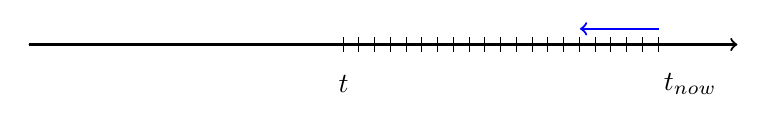
\begin{tikzpicture}[scale = 1]

\draw[thick, ->] (0,0) to (9,0);
\foreach \x in {20, ..., 40} {
  \draw[-|] (0,0) to (\x/5,0);
}

\node (t) at (8.4,-0.5) {$t_{now}$};
\node (t0) at (4,-0.5) {$t$};

\draw[thick, blue, ->] (8, 0.2) to (7,0.2);

\end{tikzpicture}


Каждый раз, когда нам нужно сделать Insert($t$, $update$) или Delete($t$, $update$), будем откатывать изменения от $t_{now}$ до $t$, затем применять новое изменение и применяем все $r$ изменений снова.
\end{proof}


\begin{theorem} 

Существует структура данных в модели straight-line-program с операциями $update$ и $query$, работающими за $\mathcal{O}(1)$, такая, что любая частично ретрактивная структура в модели history-dependent algebraic-computation-tree, integer-RAM или real-RAM будет тратить $\Omega(r)$ времени на $update$ или $query$, причем как в худшем случае, так и амортизированно.

\end{theorem}

\begin{proof}

Рассмотрим структуру, которая хранит два числа $x$ и $y$, изначально равные нулю, и поддерживает следующие операции:

\newcommand{\pluseq}{\mathrel{+}=}

\begin{itemize}

\item $x \pluseq c$
\item $y \pluseq c$
\item $y = x \cdot y$

\end{itemize}

Покажем, что эта структура нам подходит.
Для этого рассмотрим последовательность операций:

\begin{tabular}{ l }

$y \pluseq a_n$\\
$y = x \cdot y$\\
$y \pluseq a_{n - 1}$\\
$y = x \cdot y$\\
\dots\\
$y \pluseq a_0$\\
Query($t_{now}$, $y$)

\end{tabular}

\vspace{10pt}
Так мы получим значеним многочлена $a_n x^n + \dots + a_1 x + a_0$ в точке 0.

После чего сделаем ретрактивный Insert($t = -1$, "$x \pluseq c$").
Теперь Query($t_{now}$, $y$) уже дает нам значение этого многочлена в точке $c$.

И так мы можем считать значение многочлена в любой точке.

Но для вычисления многочлена в точке (при известном заранее многочлене, но неизвестной точке) есть нижняя оценка $\Omega(n)$ в любой модели из условия (\cite{frandsen2001lower}).

Таким образом, если мы сделаем достаточное количество вызовов Insert($t = -1$, "$x \pluseq c$") и Query($t_{now}$, $y$), то мы поймем, что нам потребуется $\Omega(r)$ времени на операцию даже амортизированно.
\end{proof}

